\chapter{Related Works}
\label{related works}

\section{Protocol Stack For Quantum Network}

This section discusses the protocol stack for quantum network. The protocol stack is a collection protocols that supports various levels of communication.
Here is the comparison of the protocol stack for quantum network that are presented in the previous works.

\begin{table}[ht]
  \begin{center}
    \begin{tabular}{|c|c|} \hline
       Name & Functionality \\ \hline \cline{1-2}
       Application & Run an application on an E2E connection \\ \hline \cline{1-2}
       Purification Control & Perform purification to E2E connection \\ \hline \cline{1-2}
       Entanglement Swapping Control & Perform entanglement swapping to establish an E2E connection \\
       Purification Control & Perform purification to a physical bell pair \\ \hline \cline{1-2} \hline \cline{1-2}
       Entanglement Control & Provide robustness to the bell pair establishment \\ \hline \cline{1-2} \hline \cline{1-2}
       Physical Entanglement & Establish a physical bell pair \\ \hline \cline{1-2} \hline \cline{1-2}
    \end{tabular}
    \caption{Protocol Stack for Quantum Network in \cite{Van_Meter_2009}}
  \end{center}
\end{table}

The work \cite{Van_Meter_2009} is the first study that proposed the quantum protocol stack and its proposal assumes the quantum repeater protocol that manages error using entanglement purification for both a link between two neighboring nodes and an end-to-end connection between two end nodes.
It has to be mentioned that this work assumes the number of hops for entanglement swapping and purification is assumed to be $N = 2^n$ ($n$ is a positive integer) in a linear topology. Also, this work does not assume the routing functionality in any protocol layer.

\begin{table}[ht]
  \begin{center}
    \begin{tabular}{|c|c|} \hline
      Name & Functionality \\ \hline \cline{1-2}
      Application & Run an application on an E2E connection \\ \hline \cline{1-2}
      Transport & Qubit transmission \\ \hline \cline{1-2}
      Network & Long distance entanglement \\ \hline \cline{1-2}
      Link & Robust entanglement generation \\ \hline \cline{1-2}
      Physical & Attempt entanglement generation \\ \hline \cline{1-2}
    \end{tabular}
    \caption{Protocol Stack for Quantum Network in \cite{Dahlberg_2019}}
  \end{center}
\end{table}

Another work \cite{Dahlberg_2019} proposes the different stack of quantum networking protocols that assumes the existence of transport layer that teleports a qubit using an end-to-end connection that is established by up to the network layer.
Also, it mentions the future outlook that the functionalites of routing and entanglement management may be separated from the network layer.

Although several previous works present different protocol stacks in terms of those in the upper layer, those protocol stacks still have some common features, which are 
\begin{itemize}
  \item Establishment of an actual physical Bell pair
  \item Robust entanglement generation
  \item Extension of physical bell pairs in order to establish an end-to-end Bell pair
\end{itemize}

These three elements will be the foundation of quantum network. This thesis will introduce specific protocols in the physical layer that is responsible for establishing the physical bell pair and link layer that adds robustness in the process of entanglement generation.

\section{Physical Layer Protocols For Quantum Network}

A previous work \cite{Dahlberg_2019} proposes the communication protocol for the physical layer for two of the four different use cases of a quantum network that it defines.
The protocol is called the midpoint heralding protocol (MHP) in short.

\subsubsection{MHP for Create and Keep (CK)}

Create and Keep is the use case when multiple entanglements should be stored simultaneously, such as quantum sensing \cite{PhysRevLett.109.070503}, metrology \cite{komar2014quantum} and distributed quantum computing \cite{10.1145/1060590.1060662}.
The process of entanglement generation is triggered by the reception of the message from the link layer, which includes the following parameters.
\begin{itemize}
  \item An ID for the entanglement generation attempt
  \item Generation parameters
  \item Qubits on the physical device which entanglements will be stored.
  \item The detail of microwave and laser pulse sequence
\end{itemize}

Then, the GEN message, which asks for the entanglement generation with the ID in the given message and the timestamp is sent to the support node in the middle. 
The support node uses the given timestamp to see if it receives the same IDs from the both side within a certain amount of time.
Also, it sends a REPLY message which includes the result, which is either success or failure, the generated state, and a sequence of IDs of entangled qubits after the measurement.
Then the end node performs an additional gate operation on the physical qubit depending on what state is generated, and redirected the received information to the link layer.

\subsubsection{MHP for Measure Directly (MD)}

Measure Directly is the usecase when multiple entanglements need to be created sequentially such as quantum key distribution \cite{PhysRevLett.67.661} and secure identification \cite{damgaard2007secure}.
The basic procedure is the same as the one above, but there are two main differences.  One is the operations that the end nodes perform on qubits.
Instead of performing additional state, it performs measurement on a specific basis.  The othe one is the timing of measurement. These nodes perform these measurement only they receive successful responses.

\section{Link Layer Protocols For Quantum Network}

Communication protocols for link layer have been proposed in several previous studies \cite{Van_Meter_2009,Dahlberg_2019,matsuo2019simulation}.
The biggest difference between the communication protocol for the physical layer protocol and the one for the link layer is reliability.
The former involves the process of actual entanglement generation and classical communication that triggers the process. On the other hand, the latter requires the additional classical communication that indicates the beginning and end of entanglement generation.

The first protocol \cite{Van_Meter_2009} assumes that end nodes of a physical link are directly connected via an optical fiber. First of all, multiplexed optical pulses are sent to the receiver and they are demultiplexed and measured at the receiver.
After several entanglements are generated, the ACK or NACK "keep" flags for each physical qubit are sent back to the sender.
\begin{figure}[H]
  \centerline{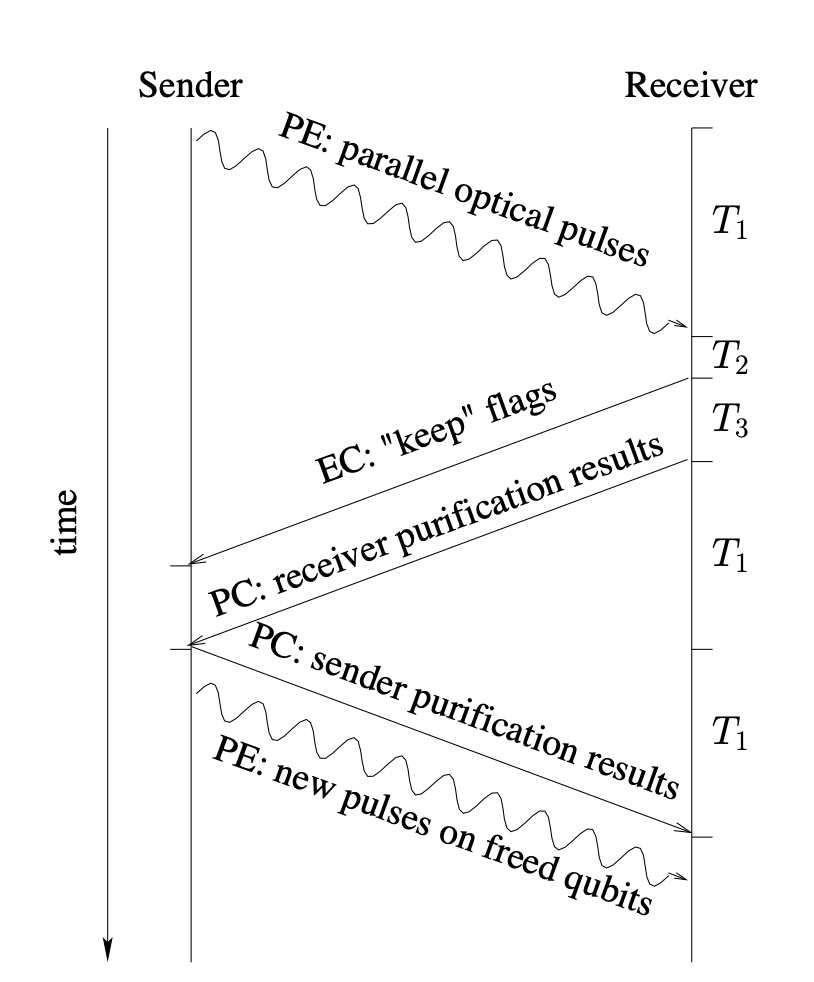
\includegraphics{images/link_protocol_rdv.jpg}}
  \caption{Message sequences in the link layer protocol in  \cite{Van_Meter_2009}}
\end{figure}

The next protocol \cite{Dahlberg_2019}
The last protocol \cite{matsuo2019simulation}
\section{RuleSet-Based Quantum Network}
